\chapter{Benchmarking Comparativo dell'Action Anticipation}

\section{Costruzione della tabella benchmark}
L'obiettivo di questo elaborato è la produzione di una tabella comparativa che raccolga i principali modelli di Action Anticipation proposti in letteratura tra il 2015 e il 2024, la quale ha richiesto un processo metodico di raccolta, normalizzazione e validazione dei dati.

\subsection{Fonti e criteri di selezione degli articoli}
\label{criteri}
Le fonti principali utilizzate per la stesura di questo elaborato sono i lavori di Hu et. al \cite{hu2022online}, Shuvo et al. \cite{shuvo2025deep} e, in particolare, il survey di Lai et al. \cite{lai2024human}, dal quale derivano la maggior parte dei risultati riportati sui vari dataset. \\
Il criterio di selezione dei modelli si basa sull'obiettivo principale del benchmark: garantire confronti validi non solo dal punto di vista quantitativo, ovvero con risultati su metriche confrontabili, ma anche dal punto di vista metodologico, richiedendo che tutti i modelli inclusi siano stati costruiti primariamente per lo stesso task.
Questo criterio nasce dalla necessità di evitare che differenze di performance dipendano dal task per cui ciascun modello è stato ottimizzato, piuttosto che dal metodo stesso, una distinzione che nei confronti esistenti in letteratura non viene sempre applicata con rigore. Sono stati pertanto selezionati solo i modelli specificatamente progettati per il task STA, escludendo modelli qualitativamente notevoli e spesso citati in letteratura che, pur riportando risultati estraibili a  $\tau$ = 1 s, non sono stati primariamente costruiti per questo task. Tuttavia, alcuni dei modelli considerati riportano risultati anche su dataset con metriche tipiche del task LTA, come MoC su 50Salads e Breakfast Actions: per questo motivo si è deciso di individuare LTA come task secondario su cui effettuare confronti equi, mantenendo separati i due gruppi.
Questo elaborato si propone, dunque, di aggiungere un maggiore livello di analisi critica alla letteratura esistente. 

\subsection{Struttura della tabella}
Per ciascun articolo, sono stati estratti e normalizzati i seguenti campi:
\begin{itemize}
    \item \textbf{Paper}: autori dell'articolo e anno di pubblicazione.
    \item \textbf{Modello}: nome del modello proposto, quando presente.
    \item \textbf{Task}: classificazione del paradigma di anticipazione adottato (STA, FIA, NAT, LTA), secondo le definizioni fornite nel Capitolo \ref{cap1}.
    \item \textbf{Dataset e Split}: dataset utilizzato per la valutazione (EK-55, EK-100, EGTEA Gaze+, Breakfast Actions, 50Salads, ecc.) e, ove disponibile, lo split specifico (Val, Test, S1, S2).
    \item \textbf{Orizzonte di anticipazione $\tau$}: espresso in secondi o come percentuale del video futuro.
    \item \textbf{Osservazione}: durata in secondi o percentuale del video osservato prima della predizione.
    \item \textbf{Metrica}: metrica di valutazione adottata (Top-5 Accuracy, Mean Top-5 Recall, Mean-over-Classes, ecc.).
    \item \textbf{Risultati}: valori numerici riportati, con separazione tra Verb, Noun e Action ove disponibile.
    \item \textbf{Input}: modalità di input utilizzate (RGB, Optic Flow, feauture pre-estratte, audio, ecc.).
    \item \textbf{Backbone e pre-training}: rete di estrazione delle feature e dataset su cui è stata pre-addestrata.
    \item \textbf{Tipo di architettura}: categorizzazione dell'approccio architetturale principale (CNN, RNN/LSTM, Transformer, ecc.).
    \item \textbf{Fonte}: provenienza del dato (articolo originale, survey).
\end{itemize}

\subsection{Validazione dei dati}
I valori numerici sono estratti primariamente dal lavoro di Lai et al. \cite{lai2024human} e validati confrontandoli con i risultati riportati dagli autori negli articoli originali. In caso di discrepanza, è stata sempre data precedenza alla fonte originale. La tabella dei confronti, nella quale sono raccolte le caratteristiche dei modelli individuati, è riportata in Appendice \ref{appendix:a}.

\section{Dalla tabella ai confronti fair}
La tabella dei confronti (Appendice \ref{appendix:a}), raccogliendo risultati eterogenei, non è direttamente utilizzabile per effettuare confronti quantitativi, dunque, si è resa necessaria la costruzione di una seconda tabella in cui raccogliere in modo sistematico i risultati numerici di ogni modello (Appendice ), dalla quale sono stati estratti quattro sottogruppi sui quali è stato possibile effettuare confronti fair, ovvero confronti in cui la differenza di performance dipende esclusivamente dal metodo e non da fattori esterni.
Le tabelle comparative del survey di Lai et al. \cite{lai2024human}, che costituiscono la fonte primaria dei risultati, raggruppano già i modelli per dataset, orizzonte e metrica; il criterio adottato in questo elaborato aggiunge a questi vincoli il requisito del task primario condiviso, come descritto in \ref{criteri}. I quattro gruppi individuati sono descritti nelle sezioni seguenti.

\subsection{Gruppo 1: STA su Epic-Kitchens 55}
Il primo gruppo di confronto rappresenta il benchmark STA più longevo e popolato della letteratura, utilizzato in modo continuativo dal 2018 al 2024 e consolidato come riferimento primario per la valutazione dell'anticipazione a breve termine in scenari egocentrici. \\ 
Le caratteristiche dei modelli individuati per questo gruppo sono le seguenti:
\begin{itemize}
    \item \textbf{Task}: STA
    \item \textbf{Dataset}: Epic-Kitchens-55
    \item \textbf{Split}: Val
    \item $\tau = 1$ s
    \item \textbf{Metrica}: Top-5 Accurracy
\end{itemize}
Sono stati individuati 14 modelli con queste caratteristiche, come mostrato nella tabella in \textbf{Figura \ref{fig:tab_ek55_val}}. \\
Tra i modelli esclusi da questo confronto figura RU-LSTM \cite{furnari2019would, furnari2020rolling}, in quanto modello costruito per il task FIA. Tuttavia, esso riporta un valore del 79.6\% per Verb, superando il massimo osservato in questo gruppo, che appartiene a MM-Transformer \cite{roy2021action}. Questo dato è un perfetto esempio di come il confronto diretto tra modelli FIA e STA non sia metodologicamente valido. Un modello FIA viene addestrato a predire l'azione futura a più orizzonti simultaneamente, ottimizzando una perdita aggregata su tutti gli intervalli. Questo significa che, al momento della predizione a $\tau$ = 1 s, il modello è stato esposto alla struttura temporale dell'intera sequenza futura durante l'addestramento, sviluppando una rappresentazione implicita più ricca della distribuzione delle azioni nel tempo. Un modello STA, al contrario, è addestrato a predire esclusivamente a un orizzonte fisso, senza questo segnale temporale aggiuntivo. Il valore di 79.6\% su Verb del modello di Furnari e Farinella \cite{furnari2019would, furnari2020rolling} non è comparabile con i valori del gruppo di confronto, in quanto non misura la stessa capacità, ma una capacità intrinsecamente facilitata dal paradigma di addestramento. \\
Un caso analogo è rappresentato dal modello di Roy e Fernando \cite{roy2022action,roy2024predicting}, il quale riporta un punteggio del 43.9\% su Action, superando tutti i modelli presenti in questo gruppo, incluso S-GEAR \cite{diko2024semantically} (43.2\%). Anche in questo caso, tuttavia, il confronto diretto non è metodologicamente valido. Un modello NAT non viene addestrato a predire un'azione ad un orizzonte temporale esplicito, ma a predire la prossima azione nella sequenza, indipendentemente da quando essa avverrà. Questo paradigma semplifica implicitamente il task: invece di dover stimare quale azione accadrà esattamente tra $\tau$ secondi, il modello deve solo identificare la transizione più probabile nella sequenza procedurale. In contesti come quello del dataset Epic-Kitchens, dove le sequenze di azioni sono fortemente regolari, questo rappresenta un vantaggio non trascurabile.
Il fatto che sia un modello FIA che un modello NAT superino numericamente i migliori modelli STA di questo gruppo di confronto non implica che essi siano architetturalmente superiori, bensì evidenzia come questi ultimi abbiano come obiettivo la risoluzione di problemi diversi. Questi casi illustrano concretamente il criterio di esclusione discusso in \ref{criteri} \\
Il grafico in \textbf{Figura \ref{fig:graf_ek55_val}} mostra che, in un confronto equo, il modello migliore su EK-55 con $\tau$ = 1 s è S-GEAR \cite{diko2024semantically}con 43.2\% Top-5 Action Accuracy, il cui contributo centrale è una supervisione semantica guidata dal linguaggio.
\begin{figure}
    \centering
    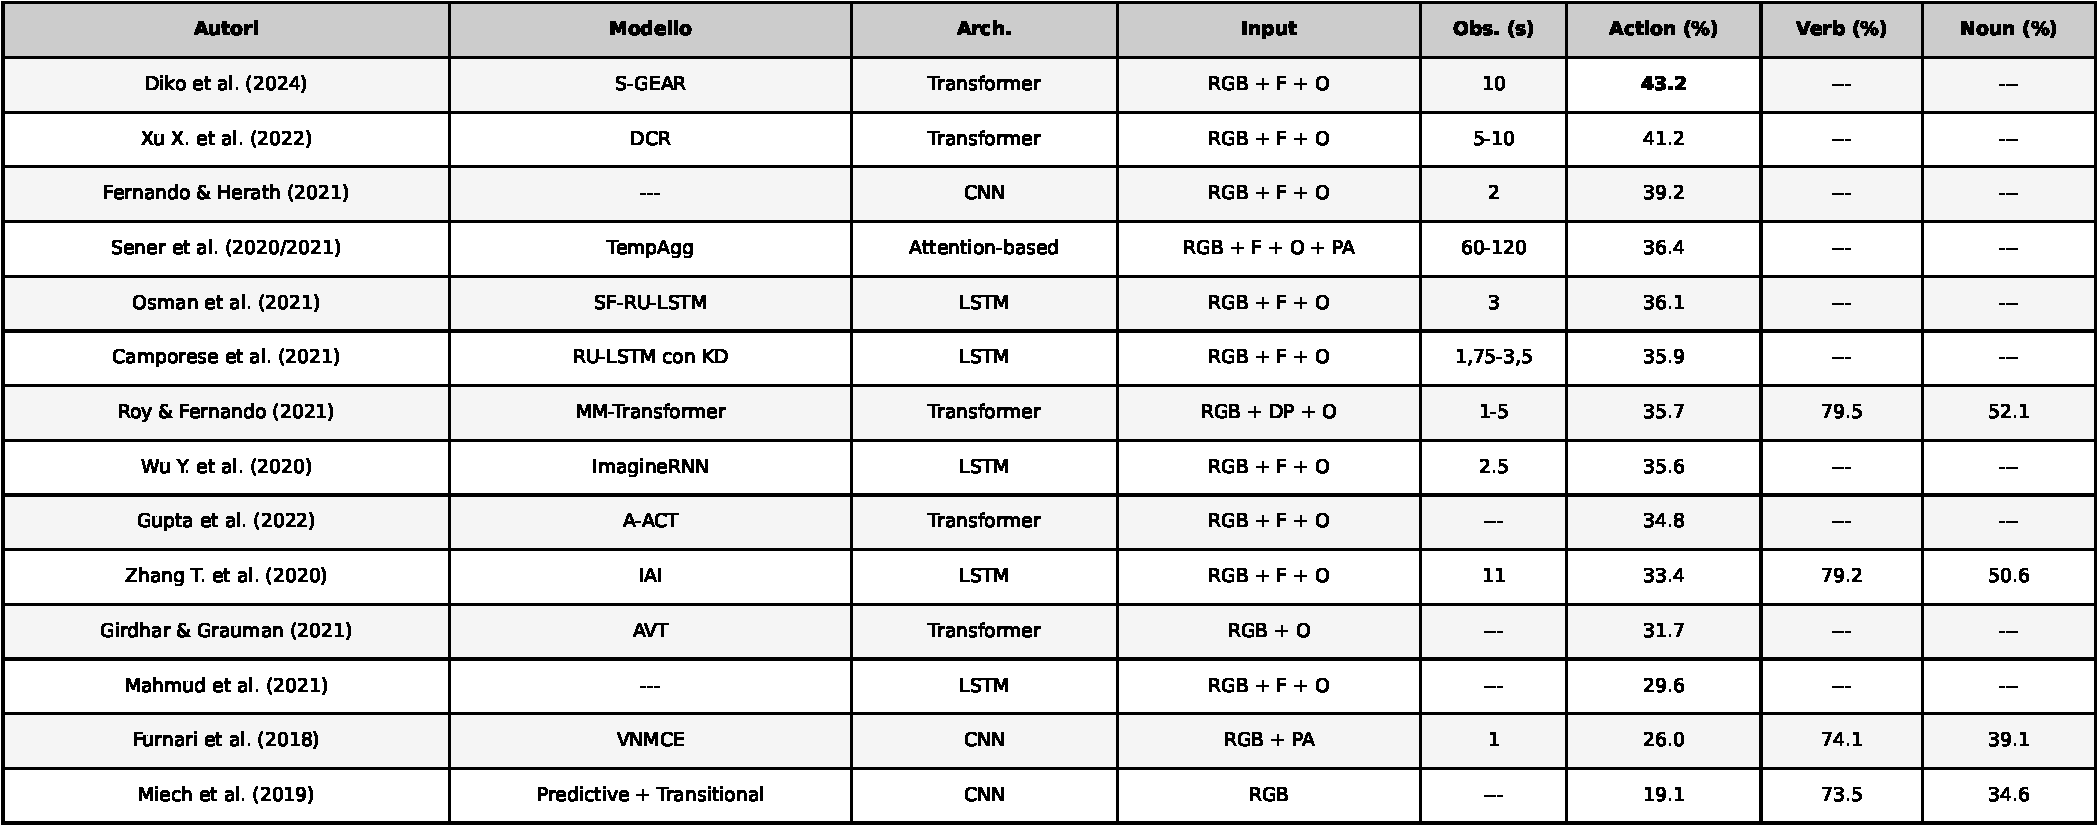
\includegraphics[width=\textwidth]{tabelle/tabella_ek55_val.pdf}
    \caption{Tabella dei modelli STA su EK-55 Val, $\tau = 1$ s,
             metrica Top-5 Accuracy.}
    \label{fig:tab_ek55_val}
\end{figure}
\begin{figure}[htbp]
    \centering
    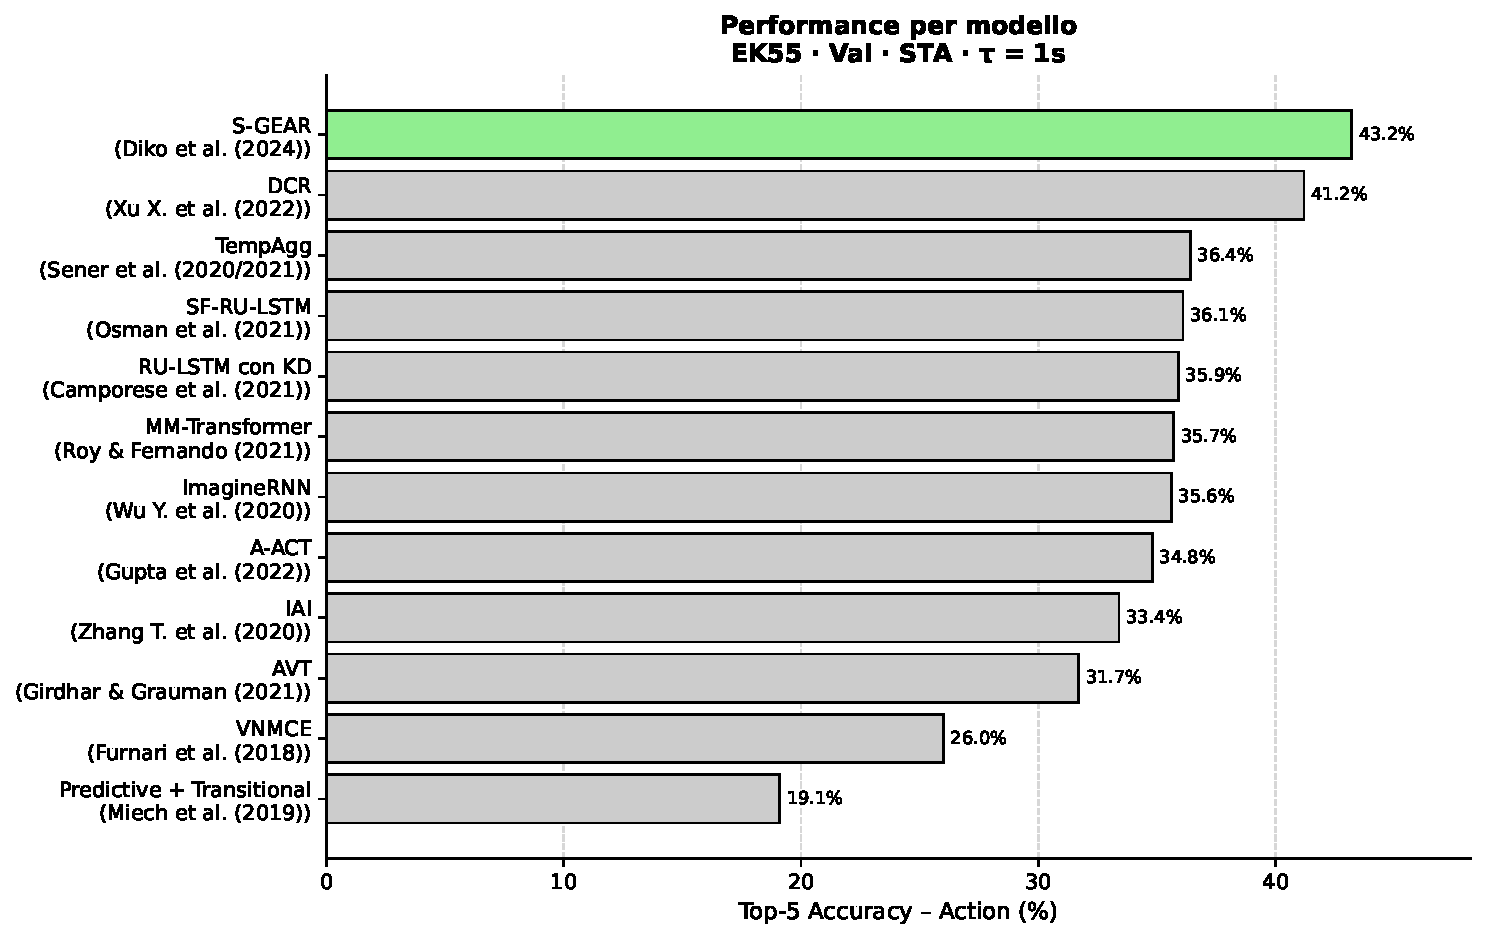
\includegraphics[width=0.85\textwidth]{grafici/barchart_ek55_val.pdf}
    \caption{Confronto delle prestazioni tra modelli STA su EK-55 Val, $\tau = 1$ s,
             metrica Top-5 Accuracy.}
    \label{fig:graf_ek55_val}
\end{figure}

\subsection{Gruppo 2: STA su Epic-Kitchens 100}
Il secondo gruppo di confronto si concentra sul dataset egocentrico più recente e sfidante della letteratura, Epic-Kitchens-100, che estende EK-55 con un numero significativamente maggiore di classi e adotta la metrica Mean Top-5 Recall, la quale penalizza in modo più equo gli squilibri tra classi frequenti e rare. Le caratteristiche dei modelli individuati per questo gruppo sono le seguenti:
\begin{itemize}
    \item Task: STA
    \item Dataset: Epic-Kitchens 100
    \item Split: Val
    \item $\tau$ = 1s
    \item Metrica: Mean Top-5 Recall
\end{itemize}
Sono stati individuati 9 modelli con queste caratteristiche, come mostrato nella \textbf{Figura \ref{fig:tab_ek100_val}.} \\
Per poter mantenere un confronto qualitativo valido, sono stati esclusi alcuni modelli che non soddisfano i criteri di uniformità del protocollo, come discusso in \ref{criteri}. %AFFT (Zhong et al., 2023) è stato escluso poiché progettato primariamente per il task \textit{Fixed Interval Anticipation} (FIA): il suo meccanismo di fusione anticipativa di feature opera su intervalli temporali fissi multipli, rendendolo non comparabile con modelli propriamente STA a orizzonte singolo. NAOGAT (Thakur et al., 2024) è stato escluso in quanto si configura come modello \textit{Next Action Prediction} (NAT), un paradigma che non impone un orizzonte temporale esplicito $\tau$. OCT (Liu S. et al., 2022) è stato infine escluso poiché l'anticipazione dell'azione costituisce solo un obiettivo secondario del modello, il cui scopo primario è la previsione della traiettoria futura delle mani. %
Il grafico in \textbf{Figura \ref{fig:graf_ek100_val}} mostra che il modello migliore è PlausiVL \cite{mittal2024can} con un punteggio di 27.6\%, seguito da InAViT \cite{roy2024interaction} con 25.9\%. AVT \cite{girdhar2021anticipative} chiude la classifica con 15.9\%.
\begin{figure}
    \centering
    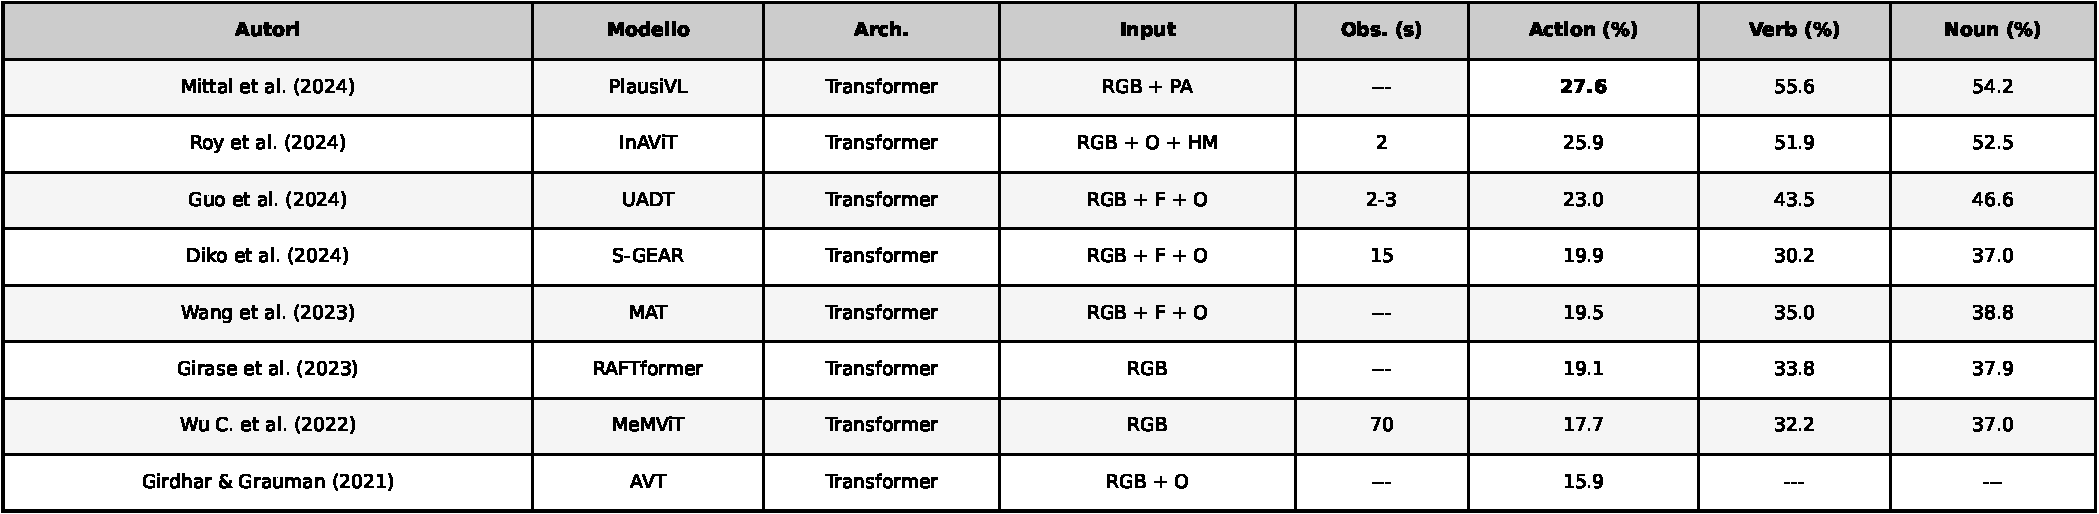
\includegraphics[width=\textwidth]{tabelle/tabella_ek100_val.pdf}
    \caption{Tabella dei modelli STA su EK-100 Val, $\tau = 1$ s,
             metrica Mean Top-5 Recall.}
    \label{fig:tab_ek100_val}
\end{figure}
\begin{figure}
    \centering
    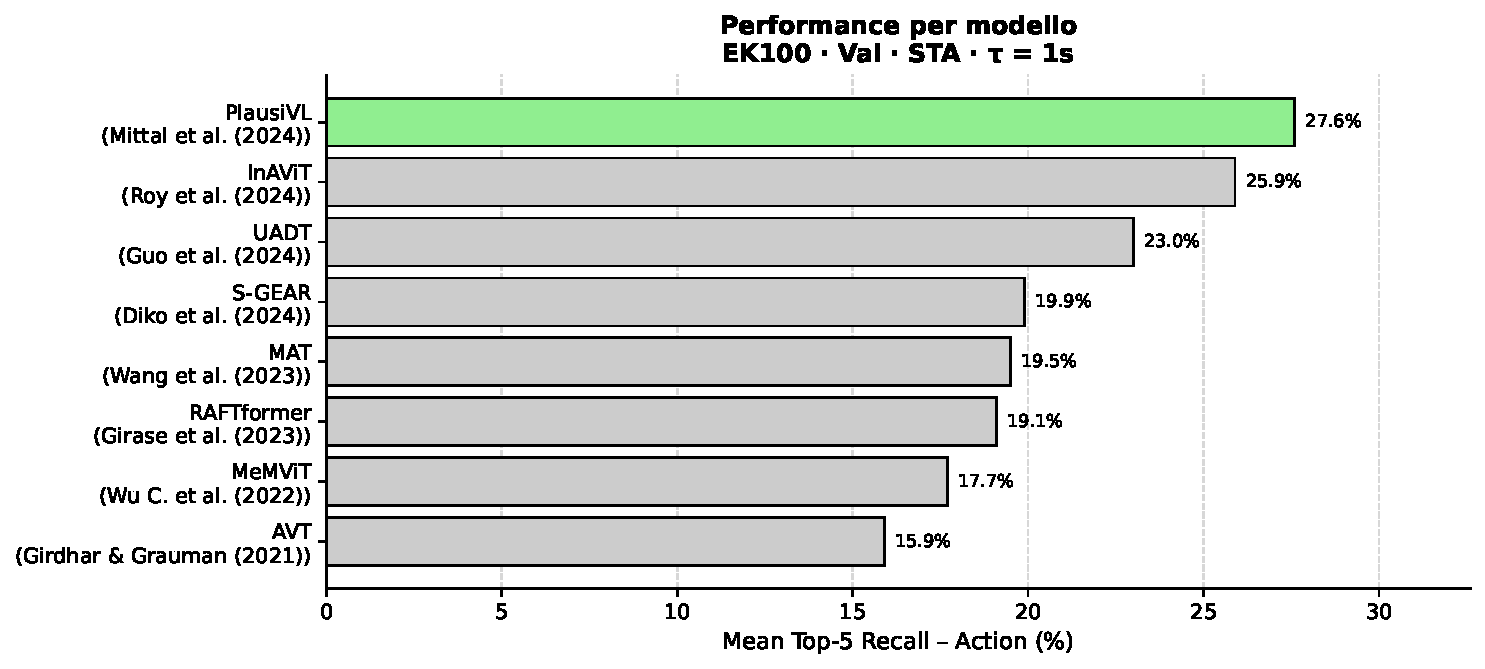
\includegraphics[width=\textwidth]{grafici/barchart_ek100_val.pdf}
    \caption{Confronto delle prestazioni tra modelli STA su EK-100 Val, $\tau = 1$ s,
             metrica Mean Top-5 Recall.}
    \label{fig:graf_ek100_val}
\end{figure}

\subsection{Gruppo 3: STA su EGTEA Gaze+}
Il terzo gruppo di confronto si concentra su un dataset egocentrico di dimensioni più contenute ma metodologicamente rilevante, EGTEA Gaze+, che si distingue per la presenza di annotazioni gaze e per un orizzonte di anticipazione ridotto a $\tau = 0.5$ s, rendendo il task più sensibile alla qualità delle feature visive immediate e alla modellazione del contesto mani-oggetti. Le caratteristiche dei modelli individuati per questo gruppo sono le seguenti:
\begin{itemize}
    \item Task: STA
    \item Dataset: EGTEA Gaze+
    \item Split: Test
    \item $\tau = 0.5$ s
    \item Metrica: Top-1 Accuracy
\end{itemize}
Sono stati individuati 4 modelli con queste caratteristiche, come mostrato nella \textbf{Figura \ref{fig:tab_egtea_test}}. \\
Per poter mantenere un confronto qualitativo valido, sono stati esclusi alcuni modelli che non soddisfano i criteri di uniformità del protocollo come discusso in \ref{criteri}. %Anche in questo caso è stato escluso AFFT (Zhong et al., 2023) costruito primariamente per il task \textit{Fixed Interval Anticipation} (FIA), con un paradigma di addestramento non comparabile con modelli STA a orizzonte singolo. Abstract Goal / Latent Goal (Roy \& Fernando, 2022/2024) è stato escluso in quanto modello \textit{Next Action Prediction} (NAT), privo di un orizzonte temporale esplicito e quindi non inseribile in un confronto fair a $\tau$ fisso.%
Il grafico in \textbf{Figura \ref{fig:graf_egtea_test}} mostra che il miglior punteggio su questo dataset è raggiunto da InAViT \cite{roy2024interaction} con 67.8\%, seguito da S-GEAR \cite{diko2024semantically} al 45.7\%, AVT \cite{girdhar2021anticipative} al 43.0\% e FHOI \cite{liu2020forecasting} al 36.6\%.
\begin{figure}
    \centering
    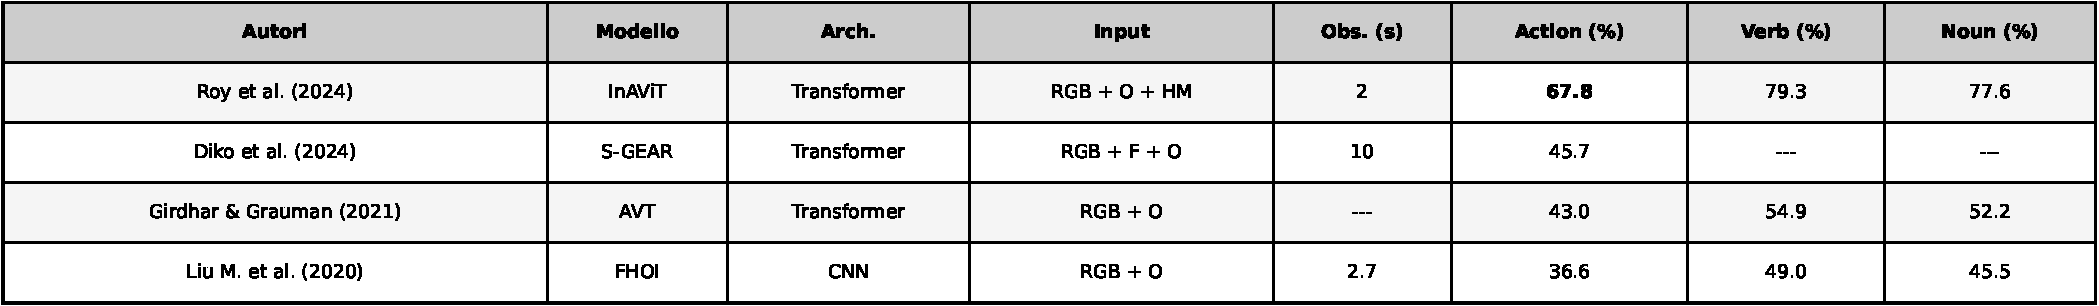
\includegraphics[width=\textwidth]{tabelle/tabella_egtea_test.pdf}
    \caption{Tabella dei modelli STA su EGTEA Gaze+ Test, $\tau = 0.5$ s,
             metrica Top-1 Accuracy.}
    \label{fig:tab_egtea_test}
\end{figure}
\begin{figure}
    \centering
    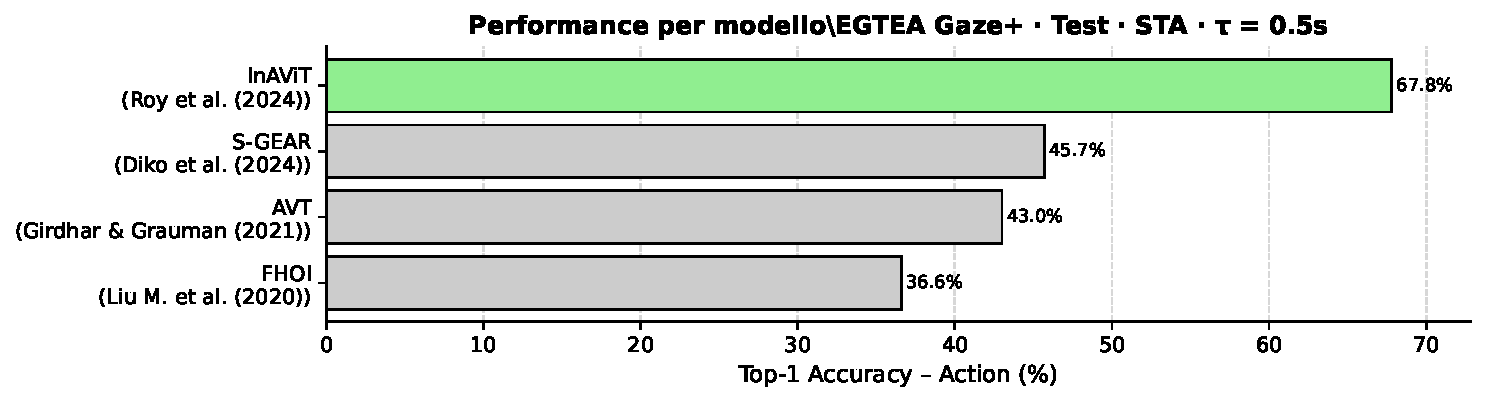
\includegraphics[width=\textwidth]{grafici/barchart_egtea_test.pdf}
    \caption{Confronto delle prestazioni tra modelli su EGTEA Gaze+ Test, $\tau = 0.5$ s,
             metrica Top-1 Accuracy.}
    \label{fig:graf_egtea_test}
\end{figure}
\subsection{Gruppo 4: LTA su Breakfast Actions}
Il quarto gruppo di confronto comprende modelli progettati primariamente per il task STA ma testati sul dataset Breakfast Actions, il quale è tipicamente associato al paradigma LTA, consentendo di analizzare la capacità di generalizzazione di architettura STA in contesti a sequenza lunga e struttura procedurale.
\begin{itemize}
    \item Task: LTA
    \item Dataset: Breakfast Actions
    \item Input: I3D Features
    \item Osservazione = 20\%
    \item Metrica: Mean-over-Classes
\end{itemize}
Sono stati individuati 3 modelli con queste caratteristiche come mostrato nella \textbf{Figura \ref{fig:tab_ba}.} \\
Per poter mantenere un confronto equo sul backbone, tutti i modelli utilizzano feature I3D pre-estratte come input. Sono stati esclusi modelli architetturalmente rilevanti come DCR \cite{xu2022learning} e S-GEAR \cite{diko2024semantically}, i quali utilizzano backbone diversi, rendendo il confronto non equo sul piano della feature extraction. Il grafico in \textbf{Figura \ref{fig:graf_ba}} mostra l'andamento delle performance dei tre modelli al variare dell'orizzonte di anticipazione. Tutti e tre i modelli mostrano una degradazione monotona al crescere dell'orizzonte. ANTICIPATR \cite{nawhal2022rethinking} si posiziona primo a tutti e quattro gli orizzonti, con valori che vanno dal 37.4\% (20\%$\to$10\%) al 28.6\% (20\%$\to$50\%). A-ACT \cite{gupta2022act} si posiziona al secondo posto con valori da 27.6\% a 21.7\%. TempAgg \cite{sener2021technical, sener2020temporal} chiude il gruppo con valori da 24.2\% a 18.1\%.
\begin{figure}
    \centering
    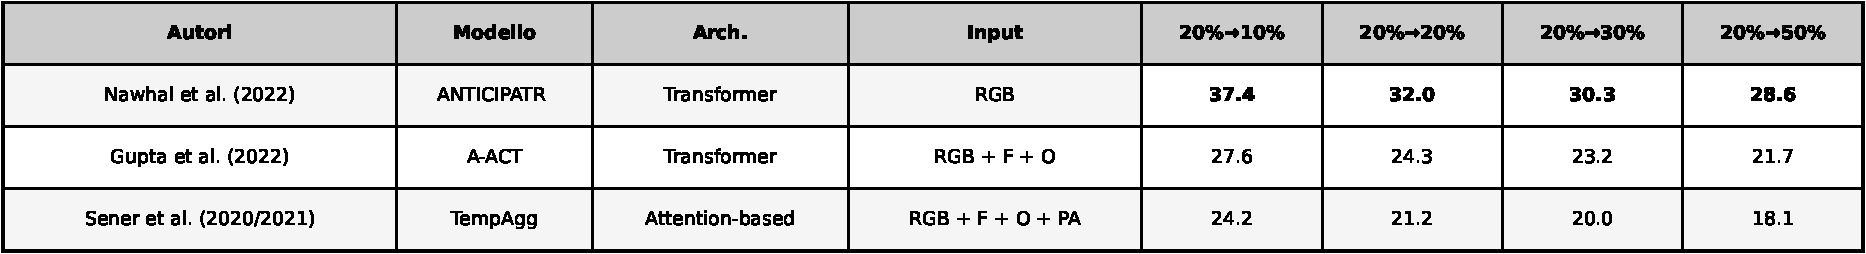
\includegraphics[width=\textwidth]{tabelle/tabella_ba.pdf}
    \caption{Tabella dei modelli LTA su Breakfast Actions, osservazione 20\%, metrica Mean-over-Classes Accuracy (MoC).}
    \label{fig:tab_ba}
\end{figure}
\begin{figure}
    \centering
    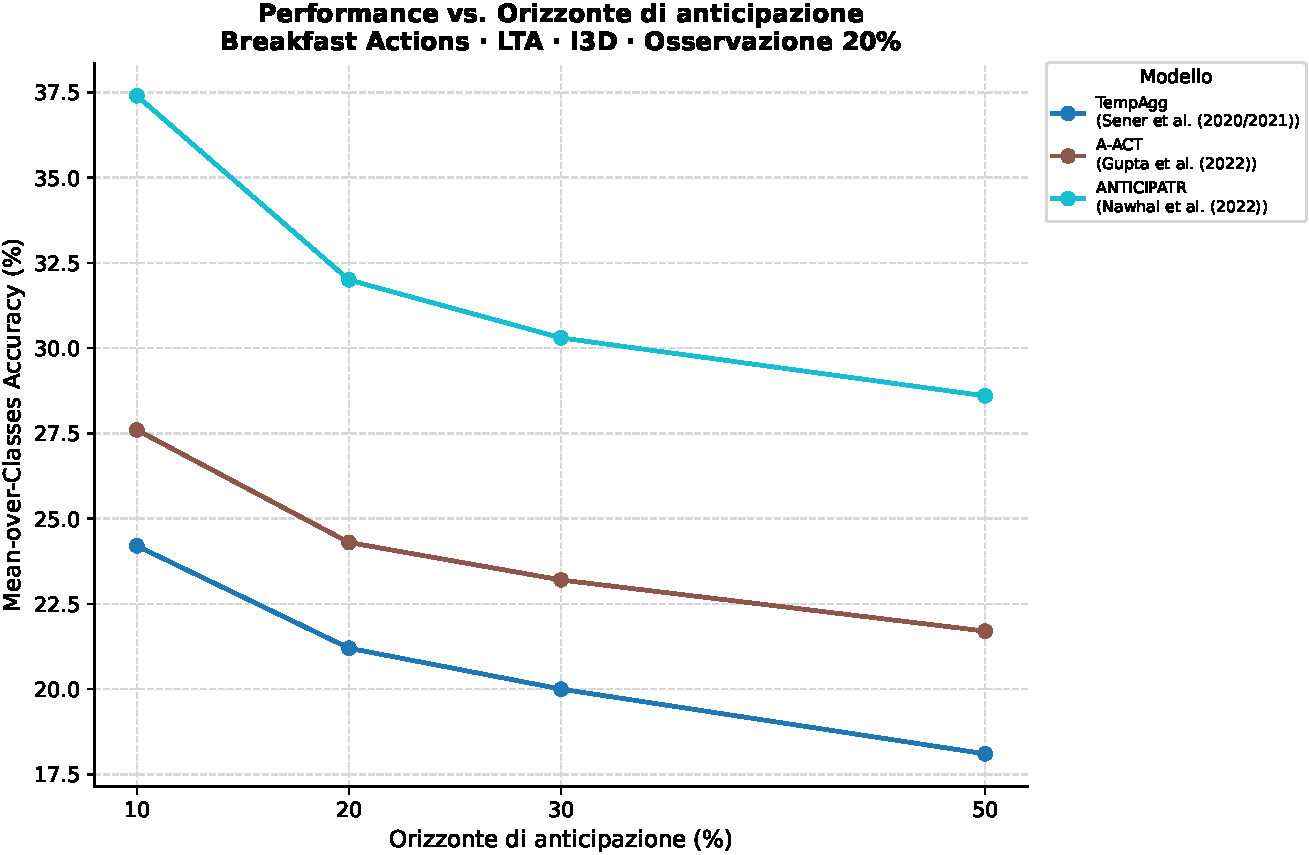
\includegraphics[width=\textwidth]{grafici/scatter_ba_performance_vs_horizon.pdf}
    \caption{Performance vs. \% orizzonte su Breakfast Action con osservazione fissata al 20\%.}
    \label{fig:graf_ba}
\end{figure}
\section{Discussione critica dei risultati}
\subsection{Multimodalità}
Dall'analisi dei quattro gruppi emerge in modo consistente che la multimodalità costituisce uno dei fattori più determinanti per le performance nel task STA. Il confronto più diretto è visibile nel Gruppo 1 (EK-55 Val): i modelli che utilizzano solo RGB si posizionano ai livelli più bassi della classifica (Miech et al. \cite{miech2019leveraging} al 19.1\% e AVT \cite{girdhar2021anticipative} al 31.7\%) mentre quasi tutti i modelli che integrano RGB con optical flow e object detections superano il 33\%. Il salto non è marginale: il solo passaggio da RGB a RGB + Flow + Object detection vale mediamente 4-5 punti percentuali, indipendentemente dall'architettura sottostante. \\
Tuttavia, il contributo delle singole modalità non è uniforme, e dipende fortemente dal tipo di informazione che ciascuna di esse aggiunge. L'optical flow cattura la dinamica del movimento ed è particolarmente utile per azioni che presentano pattern cinematici caratteristici, come tagliare e mescolare. Gli object detections forniscono informazione semantica sullo stato della scena, come ad esempio quali oggetti sono presenti e dove, indizio fondamentale e necessario per anticipare quale oggetto verrà manipolato. Il caso più estremo di questo principio si osserva nel Gruppo 3 (EGTEA Gaze+): InAViT \cite{roy2024interaction}, che integra RGB con object detections e hand masks, raggiunge un punteggio di 67.8\%, con un distacco di oltre 22 punti rispetto a S-GEAR \cite{diko2024semantically} (45.7\%), che usa RGB + Flow + Object detections ma senza localizzazione esplicita delle mani. Questo risultato suggerisce che, per dataset egocentrici ad alta densità di interazioni fisiche, la localizzazione spaziale delle mani non è una modalità accessoria ma un \textit{cue} di primo ordine. \\
Infine è importante osservare che la multimodalità ha un costo: l'optical flow è computazionalmente costoso da calcolare e memorizzare. Modelli più recenti come S-GEAR \cite{diko2024semantically} e PlausiVL \cite{mittal2024can} aggirano questo problema usando feature ViT pre-addestrate invece del flow esplicito, ottenendo risultati competitivi con un'architettura più efficiente dal punto di vista computazionale.
\subsection{Architettura}
L'evoluzione delle architetture nel periodo 2018-2024 segue un percorso non lineare, in cui l'introduzione di una nuova famiglia di modelli non sempre porta vantaggi immediati. \\
Nel Gruppo 1, i modelli CNN del periodo 2018-2020 stabiliscono le prime \textit{baseline}: VNMCE \cite{furnari2018leveraging} (26.0\%) con la sua \textit{loss} composizionale e Miech et al. \cite{miech2019leveraging} (19.1\%) con architettura multi-stream. I modelli LSTM del periodo 2020-2021 portano a un primo salto significativo, attestandosi su una base di 33-36\%: ImagineRNN \cite{wu2020learning} (35.6\%), SF-RU-LSTM \cite{osman2021slowfast} (36.1\%), RU-LSTM con KD \cite{camporese2021knowledge} (35.9\%), IAI \cite{zhang2020egocentric} (33.4\%). Il primo Trasformer del gruppo, AVT \cite{girdhar2021anticipative}, raggiunge solo 31.7\%, il che lo pone paradossalmente al di sotto delle LSTM contemporanee, confermando che il paradigma Transformer non porta vantaggi automatici su dataset di dimensioni moderate senza \textit{inductive bias} specifici per il task. Il modello TempAgg \cite{sener2021technical, sener2020temporal} (36.4\%) introduce i Temporal Aggregation Block, moduli\textit{ attention-based} in grado di aggregare rappresentazioni a scale temporali diverse, permettendo di modellare contesti fino a 120 secondi e superando le LSTM contemporanee, nonostante l'utilizzo di una struttura ricorrente.  Il salto più netto dell'intero gruppo è operato da DCR \cite{xu2022learning}(41.2\%), che non introduce una nuova architettura ma una strategia di addestramento progressivo applicabile come plug-in a qualsiasi backbone. Questo è uno dei risultati metodologicamente più rilevanti del benchmark: la strategia di training può valere più dell'architettura. S-GEAR \cite{diko2024semantically} (43.2\%) chiude il gruppo con il miglior risultato, combinando backbone ViT con rappresentazioni guidate semanticamente. \\
Nel Gruppo 2 (EK-100 Val) tutti i modelli individuati adottano un'architettura Transformer. Questo riflette un cambio di rotta nella letteratura: a partire dal 2022, i modelli basati su architetture ricorrenti hanno progressivamente lasciato spazio ai Transformer come approccio preponderante per il task STA. I due modelli al vertice della classifica, PlausiVL \cite{mittal2024can} e InAViT \cite{roy2024interaction}, sono entrambi del 2024 e integrano rispettivamente un Large Language Model e una localizzazione esplicita delle interazioni mano-oggetto. Questo segnala una nuova fase in cui il solo approccio visivo non è più sufficiente per distinguersi, e il contributo differenziante viene da componenti esterne al dominio puramente ottico. AVT \cite{girdhar2021anticipative} è nuovamente il meno performante (15.9\%), confermando la tendenza già osservata nel Gruppo 1. \\
Nel Gruppo 4, la classifica relativa tra i tre modelli rimane stabile a tutti gli orizzonti, senza inversioni di posizione al crescere della difficoltà del task. Questo suggerisce che la capacità di gestire orizzonti di predizione lunghi è una proprietà strutturale del modello. Nel caso di ANTICIPATR \cite{nawhal2022rethinking}, questa robustezza è probabilmente legata alla sua architettura che predice l'intera sequenza futura in un singolo \textit{forward pass}, evitando l'accumulo di errori tipico dei modelli che generano un'azione alla volta, ognuna condizionata sulla predizione precedente.
\subsection{Osservazione}
La finestra di osservazione è uno dei parametri meno documentati e più variabili tra i modelli analizzati, e il suo impatto sui risultati è meno intuitivo di quanto ci si potrebbe aspettare. Nel Gruppo 1, il confronto più diretto è su IAI \cite{zhang2020egocentric} (11 secondi, 33.4\%) e il modello di Camporese et al. \cite{camporese2021knowledge} (1.75-3.5 secondi, 35.9\%): una finestra tre volte più lunga non produce un vantaggio, suggerendo che il meccanismo con cui il modello usa il contesto è più determinante della sua lunghezza. Analogamente, TempAgg \cite{sener2021technical, sener2020temporal} con 60-120 secondi di contesto raggiunge il 36.4\%, posizionandosi solo 0.5 punti sopra a SF-RU-LSTM \cite{osman2021slowfast}, che utilizza 3 secondi. La spiegazione più plausibile è che oltre una certa soglia il contesto aggiuntivo porta a rendimenti decrescenti, e che l'utilità del contesto dipende dalla capacità dell'architettura di filtrare e selezionare le informazioni rilevanti. \\
Un considerevole dato è che per almeno 5 modelli su 14 appartenenti al Gruppo 1 la finestra di osservazione è descritta come variabile nei paper di riferimento. Questo rende impossibile valutare con precisione il contributo del contesto e costituisce uno dei principali problemi di riproducibilità che verranno discussi più ampiamente nella sezione successiva (\ref{riprod}). \\
Nel Gruppo 4 (Breakfast Actions, LTA), a differenza dei gruppi STA, dove l'effetto della finestra di osservazione è difficile da isolare, l'impatto dell'orizzonte di anticipazione è direttamente osservabile e quantificabile, avendo fissato l'osservazione al 20\% e fatto variare l'orizzonte tra il 10\%, 20\%, 30\% e 50\% del video futuro. Il confronto tra le curve del grafico in \textbf{Figura \ref{fig:graf_ba}}  mostra l'andamento delle performance dei tre modelli al variare dell'orizzonte di anticipazione. Il primo dato evidente è che tutti e tre i modelli mostrano una degradazione monotona al crescere dell'orizzonte, un comportamento atteso: più lontano nel futuro si vuole predire, meno informazione contestuale è disponibile per farlo con precisione. ANTICIPATR \cite{nawhal2022rethinking} perde 8.8 punti percentuali dall'orizzonte più corto a quello più lungo, A-ACT \cite{gupta2022act} ne perde 5.9 e TempAgg \cite{sener2021technical, sener2020temporal} ne perde invece 6.1. Questa differenza nel ritmo della degradazione può essere interpretata come un indicatore della robustezza strutturale del modello all'aumento dell'orizzonte, indipendentemente dal livello assoluto di partenza, sebbene tale interpretazione rimane condizionata alla scelta della finestra di osservazione adottata.
\subsection{\textit{Cues} Semantici e Obiettivi}
I modelli che integrano \textit{cues} semantici di alto livello, come rappresentazioni di oggetti, interazioni mano-oggetto e struttura linguistica delle azioni, mostrano i guadagni più consistenti nelle parti alte delle classifiche. \\
Nel Gruppo 1, MM-Trasformer \cite{roy2021action} introduce correlazione \textit{pairwise} uomo-oggetto come input al Transformer, ottenendo il 35.7\%, risultato paragonabile al 35.6\% di ImagineRNN \cite{wu2020learning}, che usa un approccio completamente diverso. Questo suggerisce che le interazioni mano-oggetto sono utili, ma il loro beneficio dipende dall'integrazione architetturale. S-GEAR \cite{diko2024semantically} raggiunge il miglior risultato (43.2\%) sfruttando la struttura semantica del linguaggio per guidare l'apprendimento delle rappresentazioni visive, riducendo la confusione tra classi visivamente simili ma concettualmente distinte. DCR \cite{xu2022learning} agisce invece a livello di addestramento: rimuovendo progressivamente il contesto di transizione durante l'addestramento costringe il modello a sviluppare rappresentazioni più robuste dell'intenzione futura. \\
Il caso più eloquente rimane InAViT \cite{roy2024interaction} nel Gruppo 3 (EGTEA Gaze+): con un punteggio di 67.8\% si pone al primo posto, staccandosi di oltre 22 punti rispetto agli altri classificati. Questo risultato non è spiegabile con la sola capacità generale del modello; la causa principale sembra essere la localizzazione esplicita delle regioni di interazioni mano-oggetto, modellata attraveso Spatial e Trajectory Cross-Attention. Il confronto con S-GEAR \cite{diko2024semantically} è particolarmente informativo: S-GEAR usa una semantica linguistica, ma non la localizzazione spaziale delle mani, e si ferma al 45.7\%. Questo suggerisce che in EGTEA Gaze+, dove le azioni sono strettamente legate alle interazioni fisiche locali, la localizzazione spaziale delle mani è un contributo più determinante della semantica linguistica.
Nel Gruppo 2 (EK-100), PlausiVL \cite{mittal2024can} (27.6\%) dimostra che la conoscenza implicita sulla struttura causale e temporale delle attività umane appresa da un LLM è trasferibile al task di anticipazione e porta benefici reali, non riducibili al solo aumento dei parametri.
\subsection{Confronto tra Dataset}
I quattro gruppi misurano capacità diverse e non sono direttamente confrontabili, sebbeno il loro confronto sia comunque informativo. \\
EK-55 e EK-100 condividono lo stesso dominio (cucina in prima persona) ma differiscono per numero di classi, distribuzione e metrica: EK-55 usa Top-5 Accuracy su circa 125 classi di azione, EK-100 usa Mean Top-5 Recall su oltre 3800 classi. La Mean Top-5 Recall penalizza maggiormente i modelli che trascurano le classi rare, rendendo EK-100 sistematicamente più difficile in valore assoluto. Osservando le prestazioni su EK-100 e EK-55, i quali sono uno l'estensione dell’altro, possiamo notare che il modello AVT \cite{girdhar2021anticipative} risulta in fondo ad entrambe le classifiche e che S-GEAR \cite{diko2024semantically} è competitivo su EK-100 (19.9\%, quarto classificato) ma raggiunge il suo risultato migliore su EK-55, dove si posiziona primo con 43.2\%. La scarsa sovrapposizione tra i modelli valutati sui due dataset rende difficili i confronti storici e suggerisce una progressiva migrazione della comunità verso EK-100 come benchmark di riferimento. \\
EGTEA Gaze+ è un dataset molto più piccolo e con caratteristiche diverse: le azioni sono più brevi, più dense e strettamente legate alle interazioni mano-oggetto. Il divario tra InAViT \cite{roy2024interaction} e gli altri modelli su EGTEA è molto più ampio rispetto a quello osservabile su EK-55 o EK-100, suggerendo che EGTEA premia in modo particolare i modelli che interpretano esplicitamente le interazioni fisiche locali. \\
Infine, Breakfast Actions, usato nel Gruppo 4 con protocollo LTA, misura capacità completamente diverse: non la precisione sulla singola azione successiva nel breve termine, bensì la coerenza della sequenza predetta su orizzonti lunghi. I modelli che eccellono su EK-55 non necessariamente performano bene su Breakfast Actions, confermando che i due task richiedono competenze distinte.

\section{Riproducibilità e requisiti minimi}
\label{riprod}
\subsection{Problemi di riproducibilità}
L'analisi comparativa dei quattro gruppi ha messo in evidenza una serie di problemi ricorrenti che limitano la riproducibilità dei risultati e la validità dei confronti in letteratura:
\begin{itemize}
    \item \textbf{Finestra di osservazione non specificata o descritta come variabile senza indicazione del range esatto}: questo rende impossibile valutare quanto contesto il modello ha a disposizione, impedendo confronti nelle stesse condizioni;
    \item \textbf{Configurazioni di input non dichiarate esplicitamente}: alcuni modelli riportano il loro risultato migliore senza specificare quale combinazione di input lo ha prodotto;
    \item \textbf{Orizzonte di anticipazione non esplicitato}: questo ha causato l’esclusione di alcuni modelli da questo benchmark, poiché non sarebbe stato possibile effettuare confronti fair, in quanto avrebbero portato a situazioni come il caso di NAOGAT \cite{thakur2024leveraging}, il quale predice TTC (time-to-contact) come output invece di usare un $\tau$ fisso, ma viene inserito nelle tabelle di confronto di Lai et al. \cite{lai2024human} con modelli con $\tau$ = 1 s, creando un precedente di confronti non equi;
    \item \textbf{Split non dichiarati o split non uniformi}: alcuni modelli riportano risultati solo su Val, altri su S1 e S2, altri su entrambi. Lo split Val di EK-55 è sistematicamente più facile degli split S1 e S2 per via della distribuzione delle classi, rendendo i confronti tra split diversi fuorvianti;
    \item \textbf{Task primario ignorato nei confronti}: survey come quello di Lai et al. \cite{lai2024human} raggruppano i modelli esclusivamente per protocollo di valutazione, (stesso dataset, stesso $\tau$ e stessa metrica) senza però tener conto del task primario per cui ciascun modello è stato progettato. Questo porta a confrontare nello stesso gruppo modelli nati per STA con modelli nati per FIA o LTA, il cui risultato a $\tau$ = 1 s è solo uno tra i molti offset testati e non è rappresentativo del contributo metodologico del modello, come nel caso di RU-LSTM \cite{furnari2019would,furnari2020rolling} e il modello di Roy e Fernando \cite{roy2022action, roy2024predicting}, entrambi esclusi dal Gruppo 1 per questa ragione. Ulteriori modelli meno performanti sono stati esclusi dagli altri gruppi di confronti per ragioni similari.
\end{itemize}

\subsection{Requisiti minimi per confronti equi}
Alla luce dei problemi identificati, si propone la seguente lista di requisiti minimi che ogni lavoro di action anticipation dovrebbe soddisfare per consentire confronti equi e riproducibili:
\begin{itemize}
    \item \textbf{Dataset} e \textbf{split} esatti;
    \item \textbf{Task} per cui il modello è stato progettato (STA, FIA, LTA, ecc.);
    \item O\textbf{rizzonte di anticipazione} $\tau$ (in secondi o percentuale) esplicitato, per ogni configurazione.
    \item \textbf{Finestra di osservazione} in secondi, percentuale, intervallo dal minimo al massimo se variabile durante l'addestramento;
    \item \textbf{Modalità di input} utilizzate con indicazione esplicita di quale combinazione produce ciascun risultato riportato;
    \item \textbf{Backbone} per l’estrazione delle feature;
    \item \textbf{Metrica} usata con formula esplicita, distinguendo se calcolata su action, verb o noun.
\end{itemize}

\section{Considerazioni finali}
L'analisi comparativa condotta sui quattro gruppi di confronto permette di trarre alcune considerazioni trasversali sui principali fattori di progresso nel campo dell'action anticipation.
\\
La multimodalità contribuisce in modo consistente: integrare più sorgenti di informazione visiva aiuta in modo solido, ma il tipo di \textit{cue} conta più della quantità. Aggiungere \textit{optical flow} e \textit{object detections} porta guadagni reali, ma la localizzazione esplicita delle interazioni mano-oggetto, come in InAViT \cite{roy2024interaction}, produce un impatto di gran lunga superiore su dataset egocentrici ad alta densità di interazioni fisiche. Non è sufficiente aumentare il numero di modalità, è necessario inoltre che il modello sappia dove guardare e come integrare le informazioni in modo strutturato rispetto al task.
\\
La strategia di training può valere più dell'architettura, ad esempio DCR \cite{xu2022learning} non introduce una nuova architettura, ma una strategia di curriculum learning applicabile come plug-in, ottenendo il singolo guadagno più significativo del Gruppo 1. Questo suggerisce che l'ottimizzazione del processo di addestramento meriti un'attenzione almeno pari alle scelte architetturali, una considerazione che la letteratura tende a sottovalutare.
\\
I Transformer non portano vantaggi automatici, diventando competitivi solo in combinazione con backbone pre-addestrati su larga scala e componenti specifici per il task, cioè memoria compressa, \textit{curriculum training}, o localizzazione delle interazioni, difatti AVT \cite{girdhar2021anticipative}, il primo modello basato su Vision Transformer per questo task, si posiziona sotto le LSTM contemporanee. 
A tal proposito è bene osservare che la semantica linguistica può contribuire anche senza ricorrere a modelli di grandi dimensioni: è il caso di S-GEAR \cite{diko2024semantically}, che dimostra che i \textit{sentence embeddings} sono sufficienti per guidare le rappresentazioni visive in modo efficace, raggiungendo il miglior risultato su EK-55.
\\
I Large Language Models (LLM) aprono una nuova fase: PlausiVL \cite{mittal2024can} raggiunge il miglior risultato nel Gruppo 2, suggerendo che il pre-training linguistico su larga scala apporti un beneficio reale per la struttura semantica delle composizioni verb-noun. Questo risultato va però interpretato con cautela: confrontare modelli con \textit{backbone} pre-addestrati su scala massiva con modelli più datati introduce variabili confondenti che i benchmark attuali non controllano sistematicamente. 
\\
Infine, la riproducibilità rimane un problema strutturale dato che la variabilità nelle configurazioni di input, nei \textit{backbone} e nelle finestre di osservazione, le quali spesso non sono documentate in modo uniforme, limita la possibilità di attribuire guadagni di performance alle scelte metodologiche corrette, rendendo ogni confronto potenzialmente fuorviante in assenza di condizioni sperimentali standardizzate.
